%%%%%%%%%%%%%%%%%%%%%%%%%%%%%%%%%%%%%%%%%%%%%%%%%%%%%%%%%%%%%%%%%
%%% %
%%% % weiiszablon.tex
%%% % The Faculty of Electrical and Computer Engineering
%%% % Rzeszow University Of Technology diploma thesis Template
%%% % Szablon pracy dyplomowej Wydziału Elektrotechniki 
%%% % i Informatyki PRz
%%% % June, 2015
%%%%%%%%%%%%%%%%%%%%%%%%%%%%%%%%%%%%%%%%%%%%%%%%%%%%%%%%%%%%%%%%%

\documentclass[a4paper, 12pt]{article}

\usepackage{weiiszablon}

\author{Brajan Miśkowicz}

% np. EF-123456, EN-654321, ...
\studentID{163976}
\grupa{EF-DI, P4}

\title{Realizacja sieci neuronowej uczonej algorytmem wstecznej propagacji błędu (learnbp) uczącej się rozpoznawania kwiatów irysa}
\titleEN{Sztuczna inteligencja - projekt}





\abstract{Treść streszczenia po polsku}
\abstractEN{Treść streszczenia po angielsku}

\begin{document}

% strona tytułowa
\maketitle

\blankpage

% spis treści
\tableofcontents

\clearpage
\blankpage

\section{Wstęp}
\subsection {Opis projektu}
Celem jest realizacja sieci neuronowej uczonej algorytmem wstecznej propagacji błędu (learnbp) uczącej się rozpoznawania kwiatów irysa. Projekt polega na napisaniu odpowiednich skryptów pozwalających na wykorzystanie sieci neuronowej - nauczenie jej rozpoznawania kwiatów irysa częścią danych - danymi uczącymi, oraz wypróbowanie działania sieci na pozostałych danych - testujących. Ponadto dzięki analizie otrzymanych z danych testowych wyników kolejnych eksperymentów należy wyznaczyć takie wartości parametrów występujących w algorytmie wstecznej propagacji, aby sieć działała możliwie najlepiej, co zostanie opisane szerzej podczas eksperymentów.

\subsection {Przedstawienie danych uczących}
Używanym zbiorem podczas projektu jest zbiór danych kwiatów irysa dostępny na stronie: \url {http://archive.ics.uci.edu/ml/datasets/Iris}. W zbiorze znajdują się cztery parametry opisujące trzy gatunki kwiatów irysa: Iris Setosa, Iris Versicolour, oraz Iris Virginica. Wśród opisu zbioru można znaleźć informacje między innymi o tym, że znajduje się w nim 150 instancji, po 50 z każdego gatunku. \\ Wspomniane wcześniej parametry opisujące kwiaty to:

- długość kielicha [cm],

- szerokość kielicha [cm],

- długość płatka [cm],

- szerokość płatka [cm].\\
W zbiorze nie pojawiają się braki danych co ułatwia ich normalizację. Na potrzeby projektu gatunki Iris Setosa, Iris Versicolour, oraz Iris Virginica zostały oznaczone podczas testów odpowiednio jako 1, 2 i 3. Z racji rozbieżności zakresów wartości parametrów danych zostały znormalizowane do zakresu wartości od -1 do 1.
\newpage
\section{Teoria}

\subsection{Neuron biologiczny}
Najważniejszym organem układu nerwowego człowieka jest mózg, który kontroluje ciało i umysł człowieka. Na podstawie wiedzy, którą dzisiaj dysponujemy można stwierdzić, że mózg
człowieka jest najbardziej złożonym obiektem we wszechświecie, jaki znamy. Komórki, z których składa się mózg, są nazywane neuronami. Każdy z neuronów za pomocą wypustek – dendrytów (gr. dendron – drzewo) może być połączony z wieloma innymi neuronami, istnieją neurony połączone z kilkoma tylko sąsiadami, ale są i takie, które mają dziesiątki tysięcy sąsiadów. Sygnały wejściowe doprowadzane są do komórki za pośrednictwem synaps, zaś sygnał wyjściowy odprowadzany jest za pomocą aksonu i jego odgałęzień, które docierają do dendrytów innych neuronów tworząc kolejne synapsy. W ten sposób każdy neuron może komunikować się z wieloma innymi, nawet odległymi neuronami. Ogólnie mówiąc, aktywność mózgu polega na generowaniu przez neurony i przesyłaniu między nimi impulsów.

\begin{figure}[hbt!]
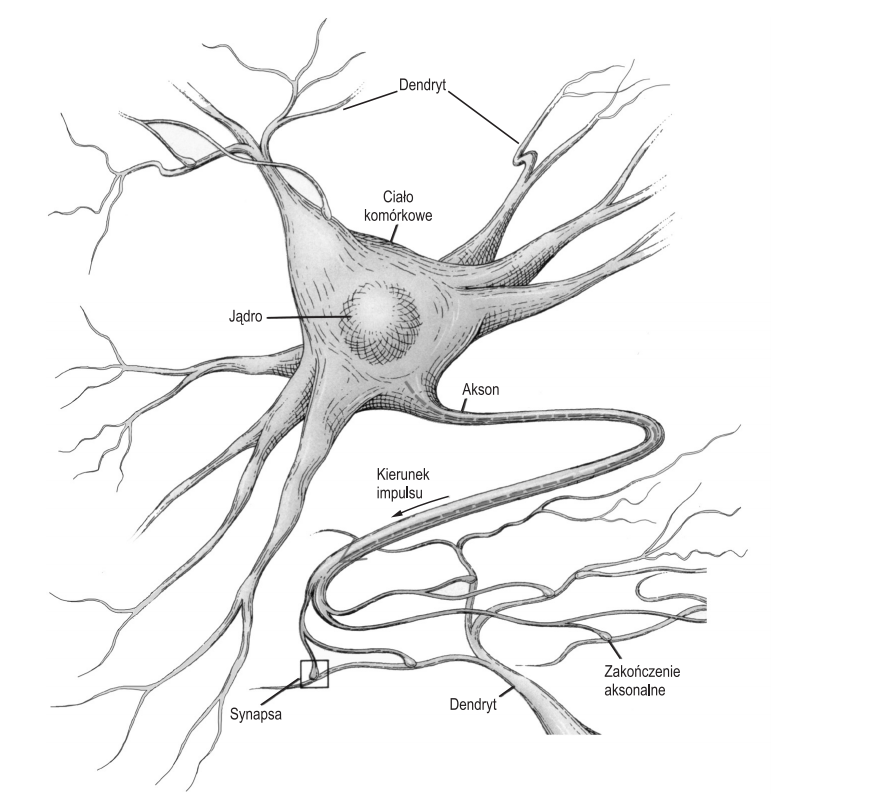
\includegraphics[width=11cm]{naturalny_neuron}
\centering
\caption{Wygląd typowego neuronu i jego części składowych\cite {book1}}
\end{figure}
\newpage
Przekazywanie impulsu nerwowego od jednej komórki do drugiej opiera się na wydzielaniu pod wpływem nadchodzących od synaps bodźców substancji chemicznych nazywanych neuromediatorami, które oddziałują na błonę komórki, powodując zmianę jej potencjału, gdzie ta zmiana jest proporcjonalna do ilości neuromediatora.
Synapsy różnią się od siebie wielkością oraz możliwościami gromadzenia tegoż neuromediatora, dlatego też impulsy docierające do neuronów za pomocą konkretnych synaps mogą powodować pobudzenia o różnej sile. Wynika z tego, że można wejściom komórki przypisać wagi, odpowiadające ilości wydzielanego jednorazowo na poszczególnych synapsach neuromediatora.\\


\subsection{Neuron sztuczny}
Podstawowym elementem sieci neuronowej jest sztuczny neuron, którego działanie wzorowane jest na funkcjonowaniu biologicznej komórki nerwowej, ale w uproszcznej formie. Pojedynczy neuron odpowiada za przetwarzanie danych wejściowych na wartość wyjściową, która jest zależna od tego, jak dany neuron reaguje na te dane. Neuron reprezentuje jednostkę przetwarzania, która przyjmuje wartość wejściową i zgodnie z określonymi regułami przekazuje inną wartość na wyjściu. Potraktować można więc każdy neuron jak  swego rodzaju procesor, który sumuje z odpowiednimi wagami sygnały wejściowe pochodzące z innych neuronów, następnie tworzy nieliniową funkcję i przekazuje tę wartość do kolejnych neuronów z nim powiązanych.

\begin{figure}[hbt!]
\includegraphics[width=12cm]{Neuron}
\centering
\caption{Budowa sztucznego neuronu\cite {book7}}
\end{figure}
Powyższy rysunek pokazuje model neuronu posiadający \textit{L} wejść \textit{x} i jedno wyjście. Najpierw sumowane są wszystkie składowe przemnożone przez ich wagi \textit{w}, a później wynik sumowania poddawany jest działaniu funkcji aktywacji, która generuje wartość na wyjściu. Nad wejściami można zauważyć tak zwane biasy, które pojawiają się na dodatkowym wejściu neuronu, mają stałą wartość - równą 1 - oznaczoną jako \textit{b} i mają za zadanie zmieniać wartość zwracaną przez neutrony tak, by sieć lepiej reprezentowała zadanie.\\
Z tą wiedzą o neuronie można zapisać wzór opisujący sztuczny neuron:

\begin{equation}
y = f \left( {\sum_{j=1}^{L}  w_j x_j + b } \right)
\label{Eq:2.1}
\end{equation}\\
\textit{y} jest tutaj wyjściem neuronu, natomiast \textit{f} oznacza funkcję aktywacji, ale można zapisać ją w prostrzy sposób traktując \textit{x} jako wektor sygnałów wejściowych oraz \textit{w} jako macierz wierszową wag\cite {book4},  tak więc:

\begin{equation}
x = [x_1, x_2, ..., x_L]^T
\label{Eq:2.2}
\end{equation}

\begin{equation}
w = [w_1, w_2, ..., w_L]
\label{Eq:2.3}
\end{equation}
oraz
\begin{equation}
y = f \left( {wx + b } \right)
\label{Eq:2.4}
\end{equation}\\

\subsection{Sieć jednokierunkowa jednowarstwowa}
Neurony połączone między sobą tworzą układ nazywany sztuczną siecią neuronową (w skrócie siecią neuronową). W zależności od sposobu połączenia neuronów można wyróżnić sieci jednokierunkowe lub rekurencyjne (ze sprzężeniem zwrotnym). Stosowana jest w tym projekcie jest jedna z najpowszechniejszych sieci - sieć jednokierunkowa.
 W sieciach jednokierunkowych przepływ sygnałów odbywa się w nich wyłącznie w kierunku od wejścia (poprzez ewentualne warstwy ukryte) do wyjścia. Wykluczony jest przepływ sygnałów w drugą stronę, co powoduje, że sieci tego typu są przeciwstawiane sieciom rekurencyjnym. Typowa sieć jednokierunkowa posiada pełne połączenia między warstwami, tj. wyjście neuronu z jednej warstwy przekazywane jest na wejście wszystkich na warstwie kolejnej. Połączenia międzywarstwowe występują jedynie między sąsiednimi warstwami.\\
 Najprostszą siecią neuronową jednokierunkową jest sieć jednowarstwowa widoczna poniżej, tworzą ją neurony ułożone w jednej warstwie. 
\begin{figure}[hbt!]
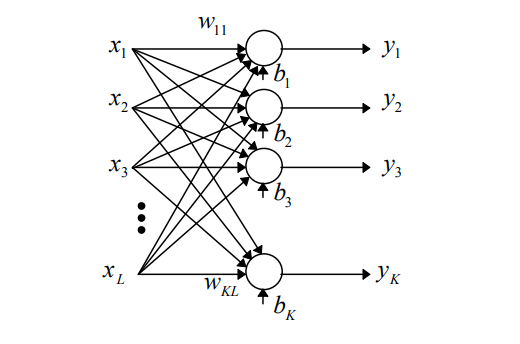
\includegraphics[width=12cm]{jednowarstwowa}
\centering
\caption{Sieć neuronowa jednowarstwowa\cite {book5}}
\end{figure}\\
Mając uzyskany wcześniej obraz neuronu i jego działania:
\begin{equation}
y = f \left( {wx + b } \right)
\label{Eq:2.5}
\end{equation}\\
można w sposób podobny zapisać jak funkcjonuje cała warstwa neuronów za pomocą tego samego wzoru, w tym przypadku jednak \textit{b} będzie wektorem przesunięć, a \textit{y} - wektorem sygnałów wyjściowych, a nie skalarami. Dodatkowo w tutaj nie będzie macierzą wierszową, a dwuwymiarową o wymiarach \textit{K} x \textit{L}, gdzie \textit{K} to liczba neuronów, a \textit{L} - liczba sygnałów wejściowych \cite{book5}:

\begin{equation}
b = [b_1, b_2, ..., b_K]^T
\label{Eq:2.6}
\end{equation}

\begin{equation}
y = [y_1, y_2, ..., y_K]^T
\label{Eq:2.7}
\end{equation}

\begin{equation}
w = 
\begin{bmatrix}
  w_{11} & w_{12} & \cdots & w_{1L} \\ 
  w_{21} & w_{22} & \cdots & w_{2L} \\ 
  \cdots & \cdots & \ddots & \cdots \\ 
  w_{K1} & w_{K2} & \cdots & w_{KL} \\ 
 \end{bmatrix}
\label{Eq:2.8}
\end{equation}

\subsection{Sieć neuronowa wielowarstwowa}
Sieć wielowarstwowa różni się od jednowarstwowej tym, że zawiera ona co najmniej jedną warstwę ukrytą.

\begin{figure}[hbt!]
\includegraphics[width=15cm]{Sieci}
\centering
\caption{Sieć jednokierunkowa wielowarstwowa\cite {book6}}
\end{figure}
Przedstawiona została powyżej sieć neuronowa wielowarstwowa, z warstwą ukrytą. Widać tutaj dokładnie to, co zostało wspomniane wcześniej - tzn. wejściem warstwy drugiej jest wyjście warstwy pierwszej, a wejściem trzeciej wyjście drugiej.\\
Mając uzyskany wcześniej wzór opisujący funkcjonowanie całej warstwy neuronów oraz wiedzę na temat budowy sieci można wyznaczyć wzory dla poszczególnych warstw - przykładowo, jak w przypadku dla trzech warstw:

\begin{equation}
y^{(1)} = f^{(1)}\left( w^{(1)}x + b^{(1)} \right)
\label{Eq:2.9}
\end{equation}

\begin{equation}
y^{(2)} = f^{(2)}\left( w^{(2)}y^{(1)} + b^{(2)} \right)
\label{Eq:2.10}
\end{equation}

\begin{equation}
y^{(3)} = f^{(3)} \left( w^{(3)}y^{(2)} + b^{(3)} \right)
\label{Eq:2.11}
\end{equation}\\
Oznaczenia tutaj są identyczne, jak wcześniej. Górne indeksy mówią natomiast, z której warstwy brane są wartości.
Po wyznaczeniu wzoru na poszczególne warstwy możliwe jest opisanie całej sieci za pomocą jednego wzoru:

\begin{equation}
y^{(3)} = f^{(3)} \left(w^{(3)} f^{(2)}\left( w^{(2)} f^{(1)}\left( w^{(1)}x + b^{(1)} \right)+ b^{(2)} \right) + b^{(3)} \right)
\label{Eq:2.12}
\end{equation}\\

\subsection{Propagacja wsteczna}
W algorytmie wstecznej propagacji najpierw obliczany jest sygnał wyjściowy, a na jego podstawie błąd warstwy wyjściowej. Następnie odwórcony zostaje kierunek przepływu sygnałów, a funkcje aktywacji zostają zastąpione przez ich pochodne, a wagi są odpowiednio aktualizowane.
Propagacja wsteczna jest metodą uczenia nadzorowanego - tzn. że dla każdego sygnału wejściowego dana jest pożądana odpowiedź.\\

\subsubsection{Uczenie pod nadzorem pojedynczej warstwy neuronów}
Każda sieć neuronowa jest przybliżeniem funkcji, więc różni się od niej o pewną wartość. Ta wartość to błąd, a naszym celem powinno być dążenie do zminimalizowania go. Ponieważ w sieci neuronowej błąd jest funkcją wag, to chcemy więc zminimalizować błędy w stosunku do wag. 
Wiedząc, że podczas uczenia każdy wektor wejściowy x posiada swój odpowiednik w postaci pożądanego wektora sygnałów wyjściowych:

\begin{equation}
x = [x_1, x_2, ..., x_L]^{T}
\label{Eq:2.13}
\end{equation}

\begin{equation}
\widehat{y} = [\widehat{y}_1, \widehat{y}_2, ..., \widehat{y}_K]^{T}
\label{Eq:2.14}
\end{equation}\\
To błąd sieci można zdefiniować następująco:

\begin{equation}
e = y - \widehat{y}
\label{Eq:2.15}
\end{equation}

\newpage
Z racji faktu, iż poszukuje się zgodności odpowiedzi \textit{y} z pożądanym wyjściem $\widehat{y}$, to cel uczenia można określić jako minimalizację pewnej funkcji, którą najczęściej jest błąd średniokwadratowy wyznaczany dla wszystkich \textit{K} neuronów:

\begin{equation}
E = \frac{1}{2} {\sum_{j=1}^{K}  e^{2}_j}
\label{Eq:2.16}
\end{equation}\\
Wzór opisujący wartość nowej wagi dla \textit{i}-tego neuronu i \textit{j}-tej wagi jest postaci: 

\begin{equation}
w_{ij}(t + 1) = w_{ij}(t) + \Delta w_{ij}(t)
\label{Eq:2.17}
\end{equation}\\
gdzie t oznacza epokę, czyli numer cyklu uczenia. Kierunek minimalizacji tworzony jest na podstawie przestrzeni wielowymiarowej w taki sposób, aby wagi podążały w kierunku punktu o najmniejszej wartości błędu. Stosowany do wyznaczenia kierunku jest wektor gradientu względem wag wszystkich warstw sieci. Zmiana wartości wag jest równa: 

\begin{equation}
\Delta w = - \eta \nabla E(w)
\label{Eq:2.18}
\end{equation}\\
gdzie $\eta$ jest współczynnikiem uczenia, a $\nabla$ gradientem wskazującym najszybszy kierunek wzrastania funkcji - z jego powodu wynika znak minusa, ponieważ zmiana \textit{w} powinna prowadzić do kierunku przeciwnego - najszybszego malenia błędu. Z poprzedniego wzoru dla tego samego jednego neuronu wynika:

\begin{equation}
\Delta w_{ij} = - \eta \frac{\partial E}{\partial w_{ij}}
\label{Eq:2.19}
\end{equation}\\
Z racji tego, że E zależne jest od wagi poprzez pobudzenie, oraz wyjście neuronu, to:

\begin{equation}
E = E(y_i(z_i(w_{ij})))
\label{Eq:2.20}
\end{equation}\\
A pochodna będzie równa:

\begin{equation}
\frac{\partial E}{\partial w_{ij}} = \frac{\partial E}{\partial y_i} \frac{\partial y_i}{\partial z_i} \frac{\partial z_i}{\partial w_{ij}}
\label{Eq:2.21}
\end{equation}\\
Korzystając z otrzymanego wcześniej wzoru na popełniany błąd i błąd średniokwadratowy można obliczyć, że:

\begin{equation}
\frac{\partial E}{\partial y_i} = \frac{\partial}{\partial y_{i}} \Big( \frac{1}{2} (y_1 - \widehat{y}_1)^{2} + ... + \frac{1}{2} (y_i - \widehat{y}_i)^{2} + ... + \frac{1}{2} (y_K - \widehat{y}_K)^{2} \Big) =  y_i - \widehat{y}_i = e_i
\label{Eq:2.22}
\end{equation}\\
Na podstawie zależności opisującej działanie neuronu natomiast:

\begin{equation}
\frac{\partial z_i}{\partial w_{ij}} = \frac{\partial}{\partial w_{ij}} \Big( w_{i1}x_1 + ... + w_{ij}x_{j} + ... + w_{iL}x_L + b_i \Big) = x_j
\label{Eq:2.23}
\end{equation}\\
Podłożyć można otrzymane pochodne cząstkowe do otrzymanej wcześniej pochodnej:

\begin{equation}
\frac{\partial E}{\partial w_{ij}} = \frac{\partial E}{\partial y_i} \frac{\partial y_i}{\partial z_i} \frac{\partial z_i}{\partial w_{ij}} = e_i \cdot \frac{\partial y_i}{\partial z_i} \cdot x_j
\label{Eq:2.24}
\end{equation}\\
Natomiast pochodną do wzoru na zmianę pojedynczej wagi:

\begin{equation}
\Delta w_{ij} =  \eta (\widehat{y}_1 - y_1) \cdot \frac{\partial y_i}{\partial z_i} \cdot x_j
\label{Eq:2.25}
\end{equation}\\
Przyjmując, że zależność $y= y(z)$ jest sigmoidalna, to ostatecznie zmiana wagi będzie równa:

\begin{equation}
\Delta w_{ij} =  \eta (\widehat{y}_1 - y_1) (1 - y_i)y_i x_j
\label{Eq:2.26}
\end{equation}\\

\newpage
\subsubsection{Uczenie pod nadzorem sieci wielowarstwowej}
Jak już wcześniej wspomniano każdy neuron posiada funkcję aktywacji, te funkcje są takie same dla neuronów konkretych warstw. Sieci jednokierunkowe wielowarstwowe w warstwach wejściowej i ukrytej najczęściej wykorzystują funkcje aktywacji typu sigmoidalnego – tansig lub logsig, ale ich minusem jest wąski zakres sygnału wyjściowego, tzn. od 0 do 1, lub -1 do 1. Z tego też powodu w wastwie wyjściowej wykorzystywana jest nie posiadająca takich ograniczeń funkcja liniowa purelin.
Funkcja błędu dla sieci wielowarstwowej przyjmuje postać:\\

\begin{equation}
	\begin{aligned}
	&E  = \frac{1}{2} {\sum_{i_3=1}^{K_3}  e^{2}_{i_3}} = \frac{1}{2} {\sum_{i_3=1}^{K_3}  \big( y^{(3)}_{i_3} - \widehat{y}_{i_3} \big)^2} =\\
	&= \frac{1}{2} {\sum_{i_3=1}^{K_3} \Big( f^{(3)} \Big( {\sum_{i_2=1}^{K_2}  w^{(3)}_{i_3 i_2}y_{i_2} + b^{(3)}_{i_3} }\Big) - \widehat{y}_{i_3} \Big)^2} =\\
	&= \frac{1}{2} {\sum_{i_3=1}^{K_3} \Big( f^{(3)} \Big( {\sum_{i_2=1}^{K_2}  w^{(3)}_{i_3 i_2}f^{(2)}\Big( {\sum_{i_1=1}^{K_1}  w^{(2)}_{i_2 i_1}y_{i_1} + b^{(2)}_{i_2} } \Big) + b^{(3)}_{i_3} }\Big) - \widehat{y}_{i_3} \Big)^2} =\\
	&= \frac{1}{2} {\sum_{i_3=1}^{K_3} \Big( f^{(3)} \Big( {\sum_{i_2=1}^{K_2}  w^{(3)}_{i_3 i_2}f^{(2)}\Big( {\sum_{i_1=1}^{K_1}  w^{(2)}_{i_2 i_1}f^{(1)} \Big( {\sum_{j=1}^{L} w^{(1)}_{i_1 j}x_j + b^{(1)}_{i_1} }  \Big) + b^{(2)}_{i_2} } \Big) + b^{(3)}_{i_3} }\Big) - \widehat{y}_{i_3} \Big)^2}
	\end{aligned}
\end{equation}\\
j = 1, ..., L to numery wejść warstwy pierwszej, a $j_1 = 1, ..., K_1;  j_2 = 1, ..., K_2;  j_3 = 1, ..., K_3; $ to numery wejść warstw pierwszej, drugiej i trzeciej.\\
Rozpoczynając od warstwy wyjściowej składniki gradientu funkcji celu względem wag neuronów poszczególnych warstw otrzymuje się przez różniczkowanie powyższej zależności:

\begin{equation}
\frac{\partial E}{\partial w_{i_{3} i_{2}}^{(3)}}=\frac{\partial E}{\partial f^{(3)}} \frac{\partial f^{(3)}\left(z_{i_{3}}^{(3)}\right)}{\partial z_{i_{3}}^{(3)}} \frac{\partial z_{i_{3}}^{(3)}}{\partial w_{i_{3} i_{2}}^{(3)}} = ( y_{i_3}-\hat{y}_{i_3} ) \frac{\partial f^{(3)}\left(z_{i_3}^{(3)}\right)}{\partial z_{i_{3}}^{(3)}} y^{(2)}_{i_2}
\label{Eq:2.28}
\end{equation}\\
gdzie łączne pobudzenie $i_3$-tego neuronu warstwy wyjściowej jest równe:

\begin{equation}
z_{i_{3}}^{(3)} = \sum_{i_2=1}^{K_2} w^{(3)}_{i_3 i_2}y_{i_2} + b^{(3)}_{i_3}
\label{Eq:2.29}
\end{equation}\\
Podkładając do poprzedniego równania zależność:

\begin{equation}
\delta^{(3)}_{i_3} = ( y_{i_3}-\hat{y}_{i_3} ) \frac{\partial f^{(3)}\left(z_{i_3}^{(3)}\right)}{\partial z_{i_{3}}^{(3)}}
\label{Eq:2.30}
\end{equation}
Otrzymane zostaje ostatecznie:

\begin{equation}
\frac{\partial E}{\partial w_{i_{3} i_{2}}^{(3)}} = \delta^{(3)}_{i_3} y^{(2)}_{i_2}
\label{Eq:2.31}
\end{equation}\\
Wyznaczyć można w podobny sposób elementy gradientu względem wag warstwy ukrytej:

\begin{equation}
	\begin{aligned}
\frac{\partial E}{\partial w_{i_{2} i_{1}}^{(2)}} & =\frac{\partial E}{\partial f^{(3)}} \frac{\partial f^{(3)}\left(z_{i_{3}}^{(3)}\right)}{\partial z_{i_{3}}^{(3)}} \frac{\partial z_{i_{3}}^{(3)}}{\partial f^{(2)}} \frac{\partial f^{(2)}\left(z_{i_{2}}^{(2)}\right)}{\partial z_{i_{2}}^{(2)}} \frac{\partial z_{i_{2}}^{(2)}}{\partial w_{i_{2} i_{1}}^{(2)}} =\\
&=\sum_{i_{3}=1}^{K_{3}}\left(y_{i_{3}}-\hat{y}_{i_{3}}\right) \frac{\partial f^{(3)}\left(z_{i_{3}}^{(3)}\right)}{\partial z_{i_{3}}^{(3)}} w_{i_{3} i_{2}}^{(3)} \frac{\partial f^{(2)}\left(z_{i_{2}}^{(2)}\right)}{\partial z_{i_{2}}^{(2)}} y_{i_{1}}^{(1)}
	\end{aligned}
\end{equation}\\
oraz wejściowej:

\begin{equation}
	\begin{aligned}
\frac{\partial E}{\partial w_{i_{1} j}^{(1)}} & =\frac{\partial E}{\partial f^{(3)}} \frac{\partial f^{(3)}\left(z_{i_{3}}^{(3)}\right)}{\partial z_{i_{3}}^{(3)}} \frac{\partial z_{i_{3}}^{(3)}}{\partial f^{(2)}} \frac{\partial f^{(2)}\left(z_{i_{2}}^{(2)}\right)}{\partial z_{i_{2}}^{(2)}} \frac{\partial z_{i_{2}}^{(2)}}{\partial f^{(1)}}\frac{\partial f^{(1)}\left(z_{i_{1}}^{(1)}\right)}{\partial z_{i_{1}}^{(1)}} \frac{\partial z_{i_{1}}^{(1)}}{\partial w_{i_{1} j}^{()}}= \\
 & =\sum_{i_{3}=1}^{K_{3}}\left(y_{i_{3}}-\hat{y}_{i_{3}}\right) \frac{\partial f^{(3)}\left(z_{i_{3}}^{(3)}\right)}{\partial z_{i_{3}}^{(3)}} \sum_{i_{2}=1}^{K_{2}} \frac{\partial f^{(2)}\left(z_{i_{2}}^{(2)}\right)}{\partial z_{i_{2}}^{(2)}} w_{i_{2} i_{1}}^{(2)} \frac{\partial f^{(1)}\left(z_{i_{1}}^{(1)}\right)}{\partial z_{i_{1}}^{(1)}} x_j
	\end{aligned}
\end{equation}\\

\newpage
\section{Eksperymenty}
\subsection{Eksperyment 1 - podział danych}
Pierwszy eksperyment polega na dobraniu optymalnego podziału danych na dane uczące oraz dane testowe. Z racji braku wyznaczonej na początku optymalnej wartości współczynnika uczenia (lr) oraz ilości neuronów na obu warstwach (S1 i S2) współczynnik uczenia został ustawiony na wartość domyślną, czyli 0.1, dlatego też dla tak dużego lr dobrana została niewielka ilość neuronów, tzn. 10 na pierwszej warstwie, oraz 9 na drugiej (ilość neuronów na warstwie pierwszej S1 musi być większa od ilości neuronów na warstwie drugiej S2).
Stworzony w programie Matlab skrypt pozwala dziesięciokrotnie nauczyć sieć metodą wstecznej propagacji \cite{str2} dla każdego podziału danych. Ilość danych uczących zmienia się w zakresie od 10\% do 90\% całości zbioru, pozostała część to dane testujące - dzięki temu otrzymany średni wynik pozwala mieć większą pewność otrzymanych wyników. 150 danych znajdujących się w pliku jest podzielone po kolei klasami po 50, aby uwiarygodnić testy za każdym powtórzeniem dane są losowane dla każdej klasy indeksy, dla których określone dane z tablicy będą testowe, lub uczące - za pomocą funkcji crossvalind z argumentem Holdout\cite{str1}. Taka metoda pozwala uniknąć sytuacji w której powtarzane kolejne eksperymenty uczą się za każdym razem na tych samych danych i testują na tych samych danych, co poprzednio, oraz sytuacji w której losuje się różna ilość danych z różnych klas, przez co klasy, z których wylosowałoby się niewiele danych do uczenia mogłaby być niedouczona w jednym eksperymencie, a w kolejnym mieć bardzo dużo danych do uczenia i osiągnąć wysoką poprawność klasyfikacji. Taka sytuacja mogłaby spowodować, że otrzymane wyniki byłyby stochastyczne nie z powodu natury sieci, lecz z powodu doboru danych, co mogłoby doprowadzić do błędnych wniosków.
W kodzie po wylosowaniu danych sieć się uczy, a poprawość klasyfikacji prezentowana jest na końcu za pomocą wykresu zależności poprawności klasyfikacji od podziału zbioru.
 
\newpage
\begin{lstlisting}[frame=single, caption=Skrypt do analizy dotyczącej wpływu podziału danych na uczenie sieci]
%wyczyszczenia środowiska i ustawienie wartości początkowych
close all; clear;
disp_freq = 100;
max_epoch = 40000;
max_fail = 10000;
load iris %wczytanie zbioru
%początkowe parametry ustawione są domyślnie
S1=10;  %ilość neuronów na pierwszej warstwie
S2=9;   %ilość neuronów na drugiej warstwie
lr = 0.1; %współczynnik uczenia
averages = zeros([1,9]);    %pusta tablica dla zmiennych
for tries = 1:1:10  %dla 10 powtórzeń
    for x = 1:9 %zbiór podzielony jest na 9 sposobów
        r = 1;
        t = 1;
        for o = 1:3 %podział zbioru na klasy
            [traind] = crossvalind('Holdout', 50, x/10);    %kroswalidacja danych
            for k = 1:50 %w każdej klasie dane są podzielone na uczące i testujące
               if (traind(k) == 1)  %jeżeli indeks jest równy jeden
                   %dana jest zapisywana do zbioru testującego
                   Ptest(:,t) = Pn(:,k+50*(o-1));
                   Ttest(1,t) = T(1,k+50*(o-1));
                   t = t + 1;   %iterowanie indeksu
               else
                   %w przeciwnym wypadku jest zapisywana do zbioru uczącego
                   Plearn(:,r) = Pn(:,k+50*(o-1));
                   Tlearn(1,r) = T(1, k+50*(o-1));
                   r = r + 1;   %iterowanie indeksu
               end
            end
        end
        net = feedforwardnet([S1, S2],'traingd');   %definicja perceptonu
        net.trainParam.epochs = max_epoch;  %maksymalna liczba epok
        net.trainParam.goal = 0.25/length(Ptest); %cel wydajności
        net.trainParam.lr = lr; %learning rate
        net.trainParam.max_fail = max_fail; %maksymalna ilość błędów walidacji
        net.trainParam.showWindow = false;  %czy pokazać okno uczenia
        net.divideParam.trainRatio=1;   %ilość danych do uczenia
        net.divideParam.valRatio=0; %ilość danych do walidacji
        net.divideParam.testRatio=0;    %ilość danych do testowania
        [net,tr] = train(net,Plearn,Tlearn); %uczenie sieci neuronowej
        u = net(Ptest); %zapisanie do u tablicy otrzymanych wyjść
        result = (1-sum(abs(Ttest-u)>=0.5)/length(Ttest))*100;  %zapisanie PK
        averages(x) = averages(x)+result;   %dodawanie PK dla kolejnycych powtórzeń
        clear Plearn; clear Ptest; clear Tlearn; clear Ttest; %zresetowanie tablic
    end
end
averages = averages/10; %wyciągnięcie  średniej PK
percents = [10, 20, 30, 40, 50, 60, 70, 80, 90];%dane do osi
plot(percents, averages);%rysowanie wykresu
title('Zależność poprawności klasyfikacji od podziału zbioru');
xlabel('wielkość zbioru uczącego [% całości zbioru]') ;
ylabel('poprawność klasyfikacji [%]');
grid;
\end{lstlisting}

\newpage
Jak widać na zamieszczonych poniżej wykresach oraz danych odpowiedni do optymalnego działania sieci jest podział, w którym 80\% to dane uczące, taki podział stosowany będzie w kolejnych eksperymentach.

\begin{figure}[ht]
	\centering
	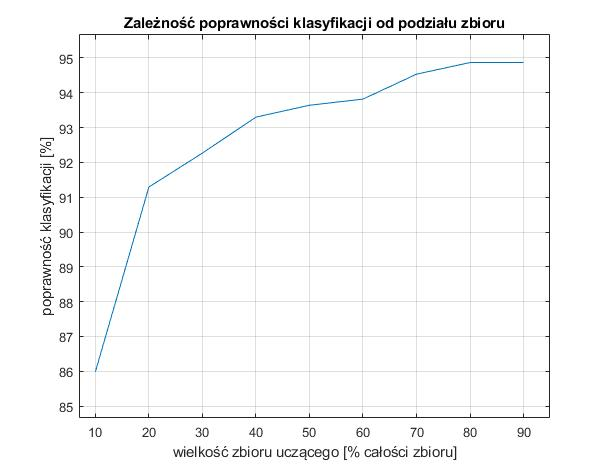
\includegraphics[width=12cm]{images/podzial1}
	\caption{Wykres zależności poprawności klasyfikacji od podziału zbioru - Pk (zbiór uczący w \%)}
\label{Fig:podzial1}
\end{figure}


\begin{figure}[ht]
	\centering
	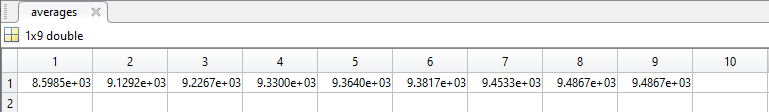
\includegraphics[width=12cm]{images/podzial1 dane}
	\caption{Dane do wykresu z rysunku 3.5 powyżej}
\label{Fig:podzial1dane}
\end{figure}

\clearpage
\subsection{Eksperyment 2 - ilość neuronów na poszczególnych warstwach}
Kod w tym eksperymencie jest podobny do poprzedniego. Wykorzystany jest już tutaj wyznaczony wcześniej podział danych. Dla każdej wartości lr = 0.1, 0.01, 0.001, 0.0001 oraz 0.00001 są w 10 powtórzeniach obliczane poprawności klasyfikacji i SSE (Sum Square Errors - suma kwadratów błędów) dla różnych ilości neuronów na pierwszej  i drugiej warstwie, pozostałe wartości w przechowującej wyniki tablicy dwuwymiarowej będące niezgodne z założeniem S1>S2 zostają zastąpione wartościami NaN, aby zapobiec ewentualnej nieczytelności wykresu.

\begin{lstlisting}[frame=single, caption=Skrypt do analizy dotyczącej wpływu ilości neuronów w obu warstwach na uczenie sieci]
%wyczyszczenia środowiska i ustawienie wartości początkowych
close all
clear
disp_freq = 100;
max_epoch = 40000;
max_fail = 10000;
load iris %wczytanie zbioru
%utworzenie potrzebnych tablic na dane i wartości
Ptest = zeros([4,30]);
Plearn = zeros([4,120]);
Ttest = zeros([1,30]);
Tlearn = zeros([1,120]);
results = zeros([11, 11]);
errors = zeros([11, 11]);

err_goal = 0.25/length(Plearn);%obliczenie pożądanej wartości błędu
j = 0;  %j to zmienna odpowiadająca za pokazywanie prograsu uczenia
lr = 1e-1;  %współczynnik uczenia, zmienian dla kolejnych eksperymentów

for tries = 1:10 %dla 10 powtórzeń
    r = 1;
    t = 1;
    for o = 1:3 %podział zbioru na klasy
        [traind] = crossvalind('Holdout', 50, 0.8);    %kroswalidacja danych
        for k = 1:50    %w każdej klasie dane są podzielone na uczące i testujące
           if (traind(k) == 1) %jeżeli indeks jest równy jeden
               %dana jest zapisywana do zbioru testującego
               Ptest(:,t) = Pn(:,k+50*(o-1));
               Ttest(1,t) = T(1,k+50*(o-1));
               t = t + 1;   %iterowanie indeksu
           else
               %w przeciwnym wypadku jest zapisywana do zbioru uczącego
               Plearn(:,r) = Pn(:,k+50*(o-1));
               Tlearn(1,r) = T(1, k+50*(o-1));
               r = r + 1;   %iterowanie indeksu
           end
        end
    end
    for S1_vec = 1:10:101   %iteracja po pierwszej warstwie neuronów
        for S2_vec = 1:10:S1_vec    %iteracja po drugiej warstwie neuronów
            j = j + 1;  %zwiększanie progresu uczenia
            net = feedforwardnet([S1_vec, S2_vec],'traingd');   %definicja percepton
            net.trainParam.epochs = max_epoch;  %maksymalna liczba epok
            net.trainParam.goal = err_goal; %cel wydajności
            net.trainParam.lr = lr; %learning rate
            net.trainParam.max_fail = max_fail; %maksymalna ilość błędów walidacji
            net.trainParam.showWindow = false;  %czy pokazać okno uczenia
            net.divideParam.trainRatio=1;   %ilość danych do uczenia
            net.divideParam.valRatio=0; %ilość danych do walidacji
            net.divideParam.testRatio=0;    %ilość danych do testowania
            [net,tr] = train(net,Plearn,Tlearn); %uczenie sieci neuronowej
            u = net(Ptest); %zapisanie do u tablicy otrzymanych wyjść
            error = sse(net, Ttest, u); %olbiczenie SSE
            pk = (1-sum(abs(Ttest-u)>=0.5)/length(Ttest))*100; %obliczenie PK
            results((S1_vec+9)/10, (S2_vec+9)/10) = results((S1_vec+9)/10, (S2_vec+9)/10) + pk;   %zapisanie do result PK
            errors((S1_vec+9)/10, (S2_vec+9)/10) = errors((S1_vec+9)/10, (S2_vec+9)/10) + error;  %zapisanie do errors SSE
            process = j/6.6;%obliczenie progresu
            fprintf('progress: %.2f%%\n', process);%wyświetlenie progresu
        end
    end
end

%wypełnienie wartościami 'NaN' pustych miejsc w tablicy (bo S2<S1)
for S2_vec = 1:10:101
    for S1_vec = 1:10:S2_vec
        results((S1_vec+9)/10, (S2_vec+9)/10) = NaN;
        errors((S1_vec+9)/10, (S2_vec+9)/10) = NaN;
    end
end

%obliczenie średnich wyników
results = results / 10;
errors = errors / 10;
SL1 = [1, 11, 21, 31, 41, 51, 61, 71, 81, 91, 101];
SL2 = [1, 11, 21, 31, 41, 51, 61, 71, 81, 91, 101];

%wyrysowanie wykresu pk
figure(1);
surf(SL1, SL2, results');
title('Zależność PK od ilości neuronów w poszczególnych warstwach');
xlabel('liczba neuronów w warstwie 1');
ylabel('liczba neuronów w warstwie 2');
zlabel('poprawność klasyfikacji [%]');
grid;

%wyrysowanie wykresu sse
figure(2);
surf(SL1, SL2, errors');
title('Zależność błędu SSE od ilości neuronów w poszczególnych warstwach');
xlabel('liczba neuronów w warstwie 1');
ylabel('liczba neuronów w warstwie 2');
zlabel('SSE');
grid;
\end{lstlisting}

\newpage
\subsubsection{Dla współczynnika uczenia lr = 0.1}\label{lr01}
Dla najwyższego współczynnika uczenia udało się znaleźć dużą ilość par parametrów S1 oraz S2, które posiadały poprawność klasyfikacji na poziomie 100\%, a sumę kwadratów błędów na poziomie 0. Najmniejsza ilość neuronów, która pozwalała osiągnąć taki wynik, to S1 = 41 i S2 = 21. Większa ilość neuronów mogłaby przeuczać sieć, ponadto sieć mogłaby się uczyć dłużej, a już te wartości dają zadowalające wyniki, dlatego też będą podstawą do późniejszych rozważań, co zostanie jeszcze opisane po kolejnych eksperymentach podczas zagęszczonych poszukiwań \ref{zageszczone}. Minimalne PK jest tutaj równe 94\%, a maksymalne SSE 2.1364.

\begin{figure}[ht]
	\centering
	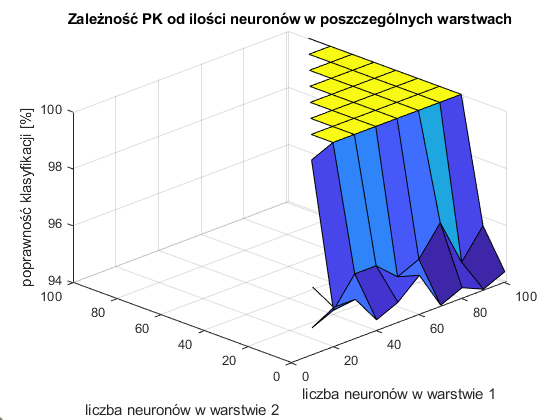
\includegraphics[width=12cm]{images/lr1 pk}
	\caption{Wykres zależności poprawności klasyfikacji od ilości neuronów w poszczególnych warstwach dla współczynnika uczenia równego 1e-1}
\label{Fig:lr1 pk}
\end{figure}

\begin{figure}[ht]
	\centering
	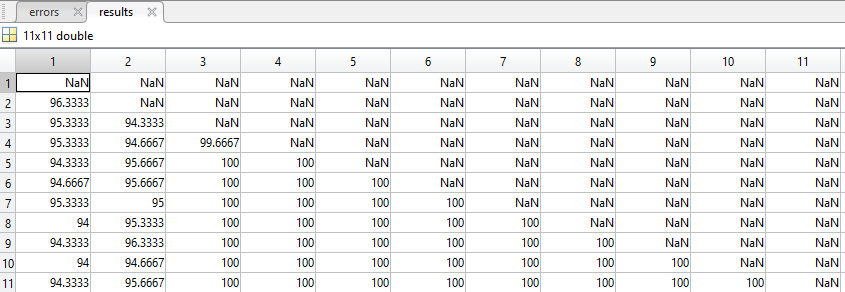
\includegraphics[width=12cm]{images/lr1 pk dane}
	\caption{Dane do wykresu z rysunku 3.7 powyżej}
\label{Fig:lr1 pk dane}
\end{figure}

\clearpage

\begin{figure}[ht]
	\centering
	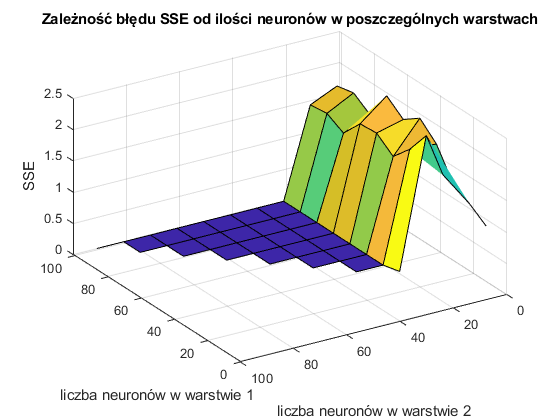
\includegraphics[width=12cm]{images/lr1 sse}
	\caption{Wykres zależności sumy kwadratów błędów od ilości neuronów w poszczególnych warstwach dla współczynnika uczenia równego 1e-1}
\label{Fig:lr1 sse}
\end{figure}

\begin{figure}[ht]
	\centering
	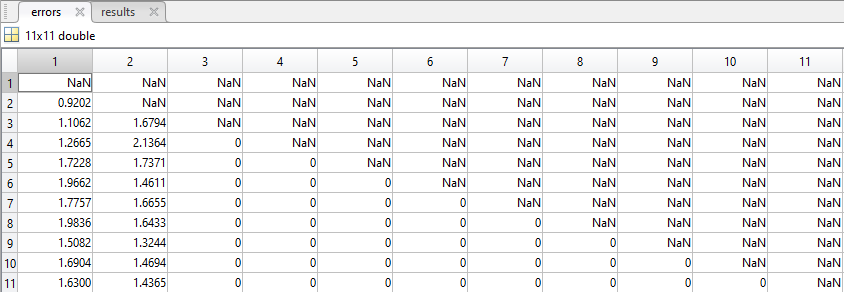
\includegraphics[width=12cm]{images/lr1 sse dane}
	\caption{Dane do wykresu z rysunku 3.9 powyżej}
\label{Fig:lr1 sse dane}
\end{figure}

\clearpage
  
\newpage
\subsubsection{Dla współczynnika uczenia lr = 0.01}
Dla mniejszego niż poprzednio współczynnika uczenia wykres traci swoje wcześniejsze właściwości, tzn. poprawność klasyfikacji nie rośnie już widocznie wraz ze wzrostem ilości neuronów, wyniki wydają się być bardziej stochastyczne w porówaniu do poprzednich, a największa poprawność klasyfikacji jest osiągana dla S1 = 31, oraz S2 = 11. Zdaje się, że większa losowość wyników pojawiaja się od 31 neuronów na drugiej warstwie wzwyż. Suma kwadratów błędów mieści się w zakresie 0.0817 - 2.0794, natomiast poprawność klasyfikacji w przedziale 92.6667 \%- 97\%.

\begin{figure}[ht]
	\centering
	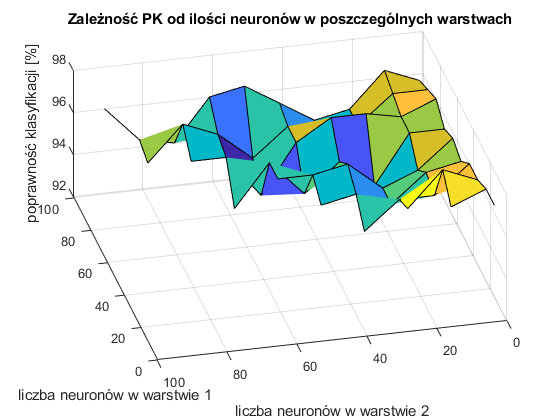
\includegraphics[width=12cm]{images/lr2 pk}
	\caption{Wykres zależności poprawności klasyfikacji od ilości neuronów w poszczególnych warstwach dla współczynnika uczenia równego 1e-2}
\label{Fig:lr1 pk}
\end{figure}

\begin{figure}[ht]
	\centering
	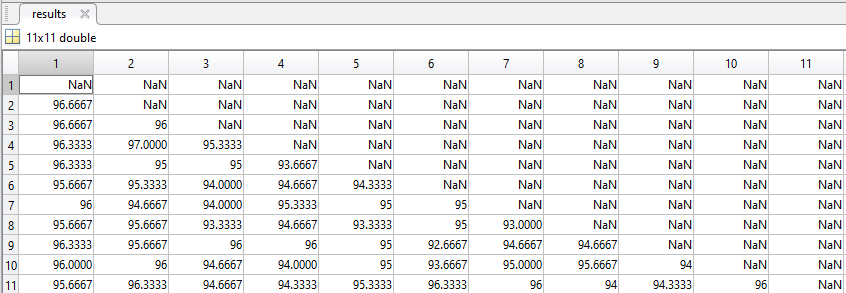
\includegraphics[width=12cm]{images/lr2 pk dane}
	\caption{Dane do wykresu z rysunku 3.11 powyżej}
\label{Fig:lr1 pk dane}
\end{figure}

\clearpage

\begin{figure}[ht]
	\centering
	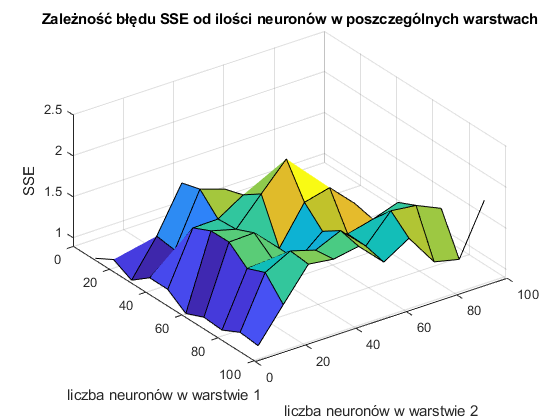
\includegraphics[width=12cm]{images/lr2 sse}
	\caption{Wykres zależności sumy kwadratów błędów od ilości neuronów w poszczególnych warstwach dla współczynnika uczenia równego 1e-2}
\label{Fig:lr1 sse}
\end{figure}

\begin{figure}[ht]
	\centering
	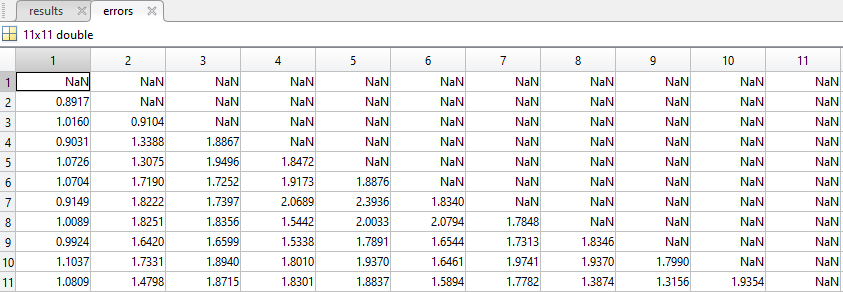
\includegraphics[width=12cm]{images/lr2 sse dane}
	\caption{Dane do wykresu z rysunku 3.13 powyżej}
\label{Fig:lr1 sse dane}
\end{figure}

\clearpage
  

\newpage
\subsubsection{Dla współczynnika uczenia lr = 0.001}
Po kolejnym zmniejszeniu współczynnika uczenia można zauważyć, że tym razem poprawność klasyfikacji maleje, a suma kwadratów błędów widocznie rośnie dla przy większej ilości neuronów - zwłaszcza na drugiej warstwie. Tym razem najlepsza poprawność klasyfikacji została otrzymana dla S1 = 21, S2 = 11. Zakres poprawności klasyfikacji to 90.6667\% - 96\%, natomiast sumy kwadratów błędów 0.9743 - 2.6305.

\begin{figure}[ht]
	\centering
	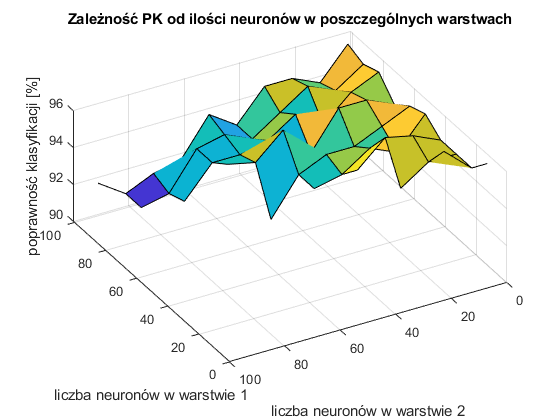
\includegraphics[width=12cm]{images/lr3 pk}
	\caption{Wykres zależności poprawności klasyfikacji od ilości neuronów w poszczególnych warstwach dla współczynnika uczenia równego 1e-3}
\label{Fig:lr1 pk}
\end{figure}

\begin{figure}[ht]
	\centering
	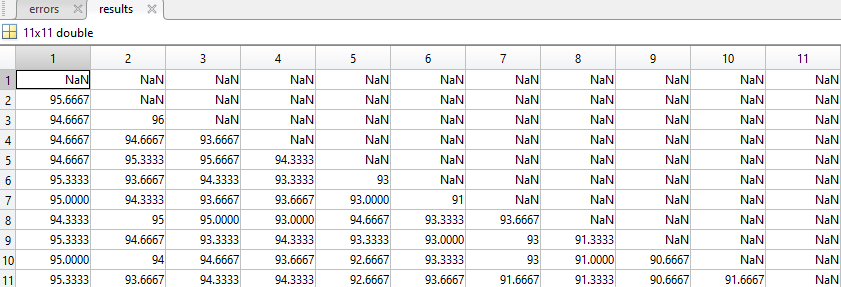
\includegraphics[width=12cm]{images/lr3 pk dane}
	\caption{Dane do wykresu z rysunku 3.15 powyżej}
\label{Fig:lr1 pk dane}
\end{figure}

\clearpage

\begin{figure}[ht]
	\centering
	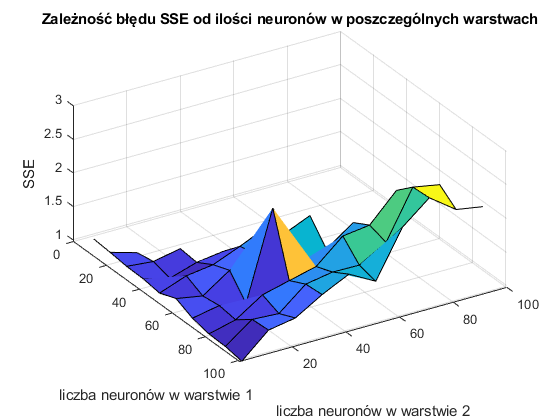
\includegraphics[width=12cm]{images/lr3 sse}
	\caption{Wykres zależności sumy kwadratów błędów od ilości neuronów w poszczególnych warstwach dla współczynnika uczenia równego 1e-3}
\label{Fig:lr1 sse}
\end{figure}

\begin{figure}[ht]
	\centering
	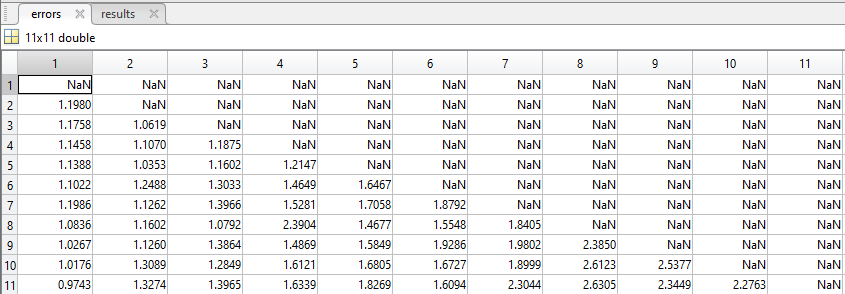
\includegraphics[width=12cm]{images/lr3 sse dane}
	\caption{Dane do wykresu z rysunku 3.17 powyżej}
\label{Fig:lr1 sse dane}
\end{figure}

\clearpage

\newpage
\subsubsection{Dla współczynnika uczenia lr = 0.0001}
Dla takiej wartości współczynnika uczenia widać, że wykresy przypominają poprzednie, nadal trend wzrostu PK i spadku SSE są podobne jak poprzednio, widać tutaj również, że dla bardzo małej ilości neuronów poprawność klasyfikacji spadła, a SSE wzrosła, jednak nie wydaje się to być istotne dla eksperymentu. Poprawność klasyfikacji mieści się w przedziale 86.3333\% - 96.6667\%, a suma kwadratów błędów 1.2877 - 4.1673.

\begin{figure}[ht]
	\centering
	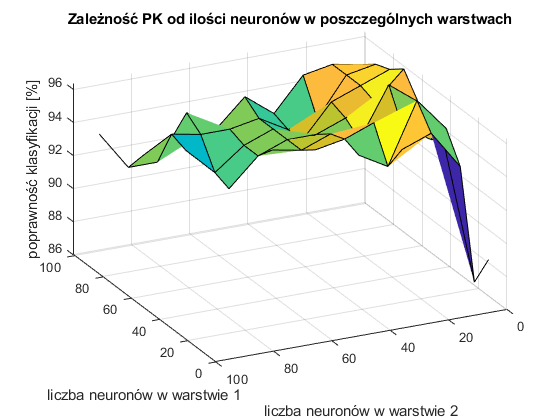
\includegraphics[width=12cm]{images/lr4 pk}
	\caption{Wykres zależności poprawności klasyfikacji od ilości neuronów w poszczególnych warstwach dla współczynnika uczenia równego 1e-4}
\label{Fig:lr1 pk}
\end{figure}

\begin{figure}[ht]
	\centering
	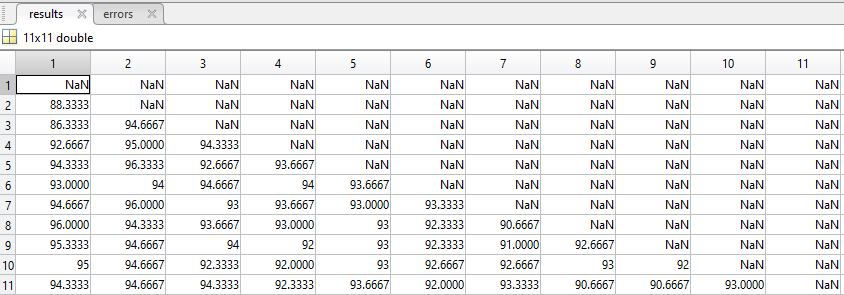
\includegraphics[width=12cm]{images/lr4 pk dane}
	\caption{Dane do wykresu z rysunku 3.19 powyżej}
\label{Fig:lr1 pk dane}
\end{figure}

\clearpage

\begin{figure}[ht]
	\centering
	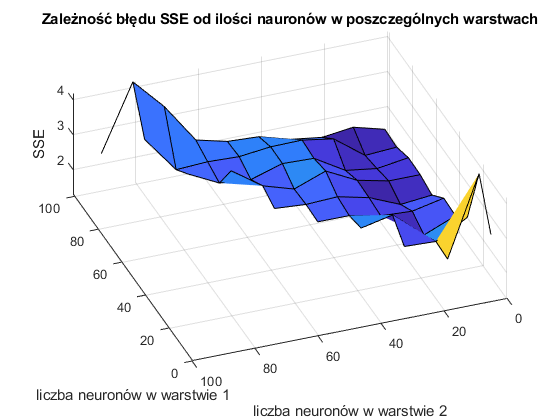
\includegraphics[width=12cm]{images/lr4 sse}
	\caption{Wykres zależności sumy kwadratów błędów od ilości neuronów w poszczególnych warstwach dla współczynnika uczenia równego 1e-4}
\label{Fig:lr1 sse}
\end{figure}

\begin{figure}[ht]
	\centering
	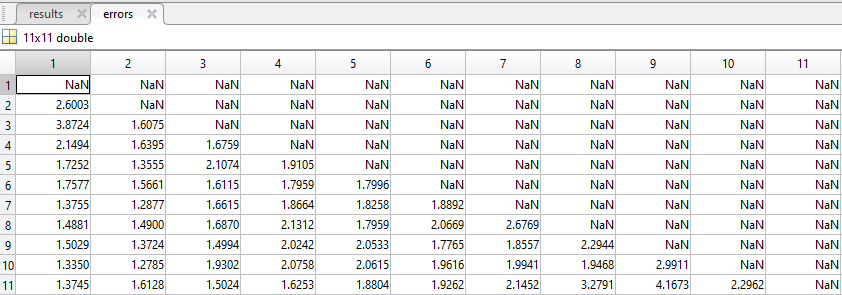
\includegraphics[width=12cm]{images/lr4 sse dane}
	\caption{Dane do wykresu z rysunku 3.21 powyżej}
\label{Fig:lr1 sse dane}
\end{figure}

\clearpage

\newpage
\subsubsection{Dla współczynnika uczenia lr = 0.00001}
Dla najmniejszej wartości  współczynnika uczenia można zauważyć, że  zgodnie z oczekiwaniami wartości poprawności klasyfikacji są wyraźnie mniejsze, a SSE większe, niż wcześniej. Co więcej Pk jest najmniejsze, a SSE największe ze wszystkich eksperymentów. Nadal jednak poprawność klasyfikacji jest największa, a sumy kwadratów błędów najmniejsze dla ilości neuronów 11-31 w drugiej warstwie.
Zakres Pk to 40.6667\% - 92.6667\%, natomiast SSE 2.1336 - 14.9306. W porównaniu do poprzednich te zakresy są spore, można więc uznać, że stochastyczność rośnie wraz z zmniejszaniem się współczynnika uczenia.

\begin{figure}[ht]
	\centering
	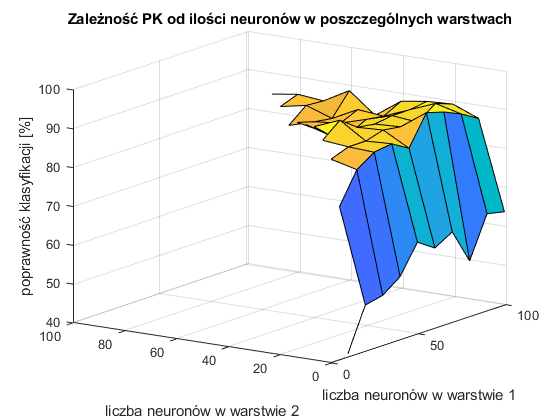
\includegraphics[width=12cm]{images/lr5 pk}
	\caption{Wykres zależności poprawności klasyfikacji od ilości neuronów w poszczególnych warstwach dla współczynnika uczenia równego 1e-5}
\label{Fig:lr1 pk}
\end{figure}

\begin{figure}[ht]
	\centering
	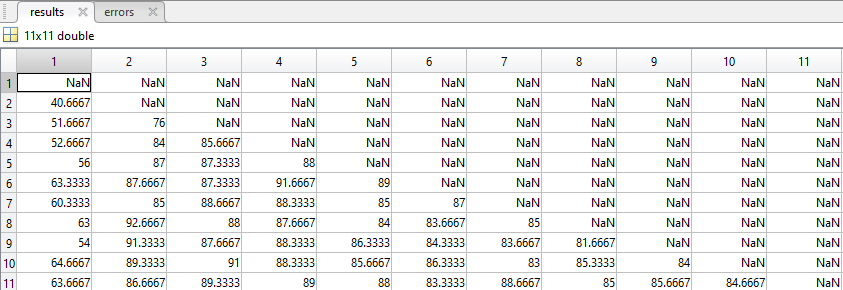
\includegraphics[width=12cm]{images/lr5 pk dane}
	\caption{Dane do wykresu z rysunku 3.23 powyżej}
\label{Fig:lr1 pk dane}
\end{figure}

\clearpage

\begin{figure}[ht]
	\centering
	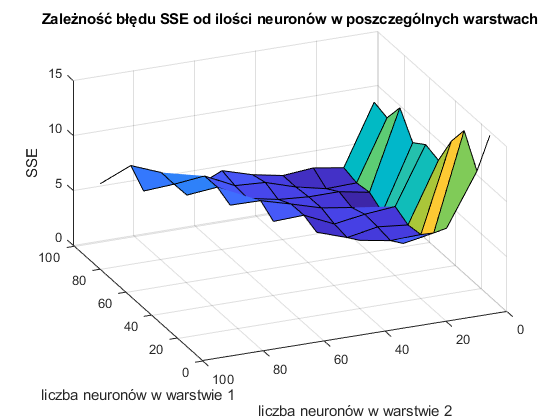
\includegraphics[width=12cm]{images/lr5 sse}
	\caption{Wykres zależności sumy kwadratów błędów od ilości neuronów w poszczególnych warstwach dla współczynnika uczenia równego 1e-5}
\label{Fig:lr1 sse}
\end{figure}

\begin{figure}[ht]
	\centering
	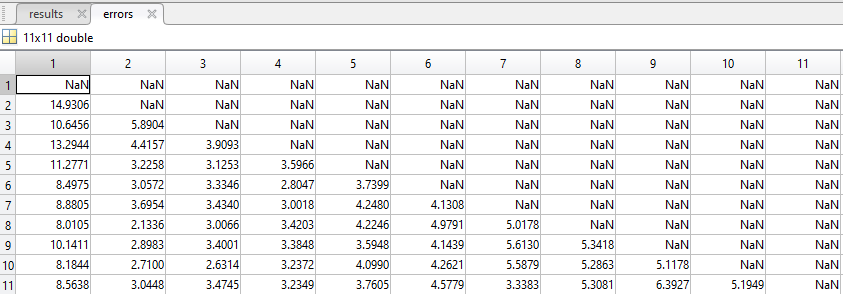
\includegraphics[width=12cm]{images/lr5 sse dane}
	\caption{Dane do wykresu z rysunku 3.25 powyżej}
\label{Fig:lr1 sse dane}
\end{figure}

\clearpage

\newpage
\subsubsection{Zagęszczone poszukiwania}\label{zageszczone}
Przy ogólnym poszukiuwaniu \ref{lr01} najbardziej zadowalające wartości poprawności i błędu zostały osiągnięte przy współczynniku lr = 0.1 i ilości neuronów na pierwszej oraz drugiej warstwie: S1 = 41, S2 = 21. Kolejny eksperyment jest rozszerzeniem wspomnianego badania, tym razem zostaje jednak zawężony zakres poszukiwań, z zakresu S1 = 11, 21, ..., 101 do S1 = 31, 32, ..., 41 oraz z S2 = 1, 11, ..., S1 do  S2 = 11, 12, ..., 21. Taki zakres poszukiwań pozwala na znalezienie mniejszej wartości neuronów, dla których sieć osiąga minimalny błąd, dzięki czemu można zredukować ryzyko przeuczenia, oraz zmniejszyć czas uczenia sieci. Kod jest tutaj niemalże identyczny, jak wcześniej, zmienione są jedynie ilości neuronów oraz tablice do przechowywania wyników.
Okazuje się, że udało się znaleźć zadowalające kombinacje liczb neuronów w obu warstwach. Z otrzymanych wyników można odczytać, że potrzebne jest 21 neuronów w drugiej warstwie, a na pierwszej wystarczy ich 36. Dodatkowo można zauważyć, że poprawność klasyfikacji rośnie, a suma kwadratów błędów maleje dla kolejnych wartości S2 szybciej, niż dla kolejnych rosnących wartości S1. Same wartości PK nie spadają poniżej 93.3333\%, a SSE nie osiąga wartości większej, niż 2.8768.


\begin{figure}[ht]
	\centering
	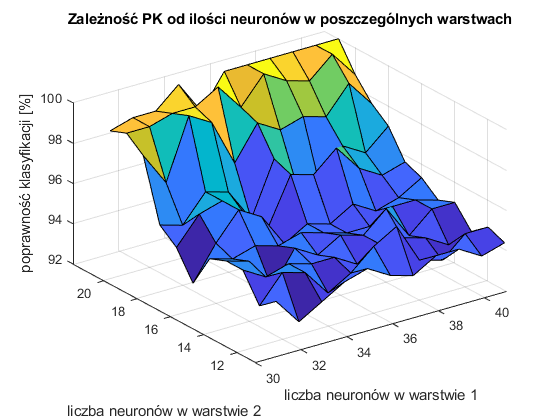
\includegraphics[width=14cm]{s1s2 pk}
	\caption{Wykres zależności poprawności klasyfikacji od ilości neuronów w poszczególnych warstwach dla współczynnika uczenia równego 1e-1 przy zagęszczonych poszukiwaniach}
\label{Fig:lr1 sse dane}
\end{figure}


\begin{figure}[ht]
	\centering
	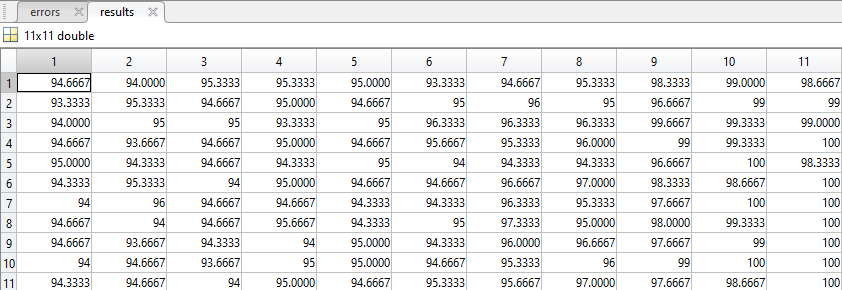
\includegraphics[width=10cm]{s1s2 pk dane}
	\caption{Dane do wykresu z rysunku 3.27 powyżej}
\label{Fig:lr1 sse dane}
\end{figure}

\begin{figure}[ht]
	\centering
	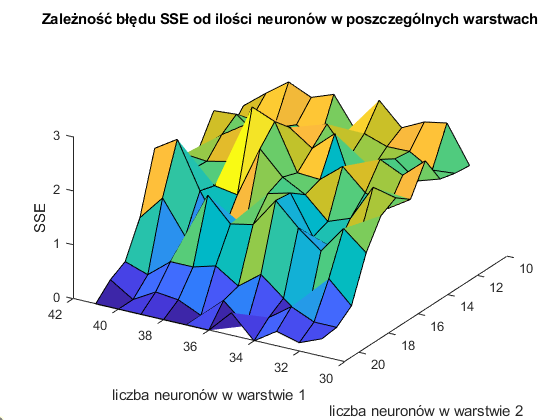
\includegraphics[width=14cm]{s1s2 sse}
	\caption{Wykres zależności sumy kwadratów błędów od ilości neuronów w poszczególnych warstwach dla współczynnika uczenia równego 1e-1 przy zagęszczonych poszukiwaniach}
\label{Fig:lr1 sse dane}
\end{figure}

\begin{figure}[ht]
	\centering
	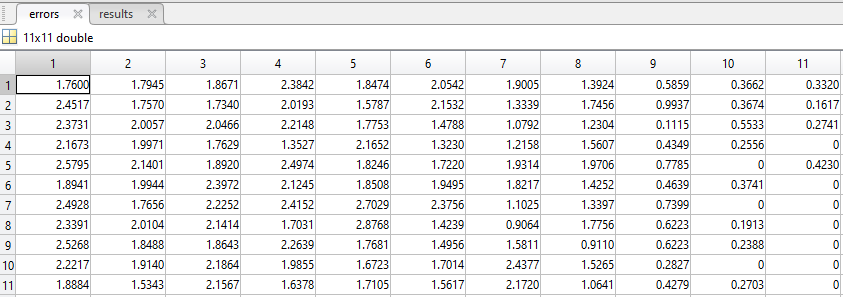
\includegraphics[width=10cm]{s1s2 sse dane}
	\caption{Dane do wykresu z rysunku 3.29 powyżej}
\label{Fig:lr1 sse dane}
\end{figure}



\clearpage

\newpage
\subsection{Eksperyment 3 - wielkość parametru współczynnika uczenia}
W tym eksperymencie badany jest wpływ współczynnika uczenia na poprawność klasyfikacji oraz sumę kwadratów błędów. Współczynnik mieści się w takim samym zakresie, jak wcześniej: lr = [1e-5, 1e-4, 1e-3, 1e-2, 1e-1]. Aby otrzymać ogólny obraz wpływu współczynnika uczenia badany jest w pierwszym z eksperymentów tego dotyczącym jak zmienia się Pk i SSE w zależności od lr, jeżeli wynik dla danego lr jest brany dla każdej możliwej pary S1 i S2, gdzie S1 = 11, 21, ..., 101; a S2 = 1, 11, ..., S1. Drugi z eksperymentów pokazuje jak zmieniają się wyniki w zależności od współczynnika uczenia dla wyznaczonej w zagęszczonych poszukiwaniach pary liczb S1 i S2.\\

\subsubsection{Współczynnik uczenia przy średniej ze wszystkich kombinacji ilości neuronów}
Zostały tutaj wykorzystane tablice z wynikami eksperymentów, w których poszukiwane były wartości S1, S2 dla różnych lr. Z eksperymentu, gdzie lr = 1e-1 wzięte są tablice results1 oraz errors1, dla lr = 1=e-2 tablice results2 i errors2, itd. Następnie wartości z tablic sumowane tak, aby result1 posiadało sumę poprawności klasyfikacji wszystkich par S1 i S2 dla lr=1e-1, podobnie error1 sumę SSE i tak dalej dla każdej tablicy. Po zsumowaniu obliczona zostaje średnia i wyrysowane są wykresy.

\clearpage

\begin{lstlisting}[frame=single, caption=Skrypt do analizy dotyczącej wpływu wartości współczynnika uczenia na uczenie sieci]
for x = 2:1:11 %dla indeksów odpowiadających S1
    for y = 1:1:x-1	%dla indeksów odpowiadających S2
       %sumowane są kolejne wartości Pk i SSE dla każdego lr
        result1 = result1 + results1(x, y);
        result2 = result2 + results2(x, y);
        result3 = result3 + results3(x, y);
        result4 = result4 + results4(x, y);
        result5 = result5 + results5(x, y);
        error1 = error1 + errors1(x, y);
        error2 = error2 + errors2(x, y);
        error3 = error3 + errors3(x, y);
        error4 = error4 + errors4(x, y);
        error5 = error5 + errors5(x, y);
    end
end
%obliczenie średniej
result1 = result1 / 55;
result2 = result2 / 55;
result3 = result3 / 55;
result4 = result4 / 55;
result5 = result5 / 55;
error1 = error1 / 55;
error2 = error2 / 55;
error3 = error3 / 55;
error4 = error4 / 55;
error5 = error5 / 55;
%tablice potrzebne do osi
range = [1e-5, 1e-4, 1e-3, 1e-2, 1e-1];
results = [result5, result4, result3, result2, result1];
errors = [error5, error4, error3, error2, error1];
%wyrysowanie wykresów
figure(1);
plot(range,results);
title('Zależność poprawności klasyfikacji od współczynnika uczenia');
xlabel('współczynnik uczenia lr');
ylabel('poprawność klasyfikacji [%]');
grid;

figure(2);
plot(range,errors);
title('Zależność błędu SSE od współczynnika uczenia');
xlabel('współczynnik uczenia lr');
ylabel('SSE');
grid;
\end{lstlisting}

\clearpage
Z otrzymanych wyników można wywnioskować, że w tym przypadku wraz ze wzrostem współczynnika uczenia rośnie poprawność klasyfikacji, oraz maleje suma kwadratów błędów. Dla kolejnych coraz mniejszych wartości lr poprawność klasyfikacji coraz gwałtowniej maleje. Dla największej wartości lr = 0.1 poprawność klasyfikacji nie osiąga 100\%, a SSE 0.


\begin{figure}[ht]
	\centering
	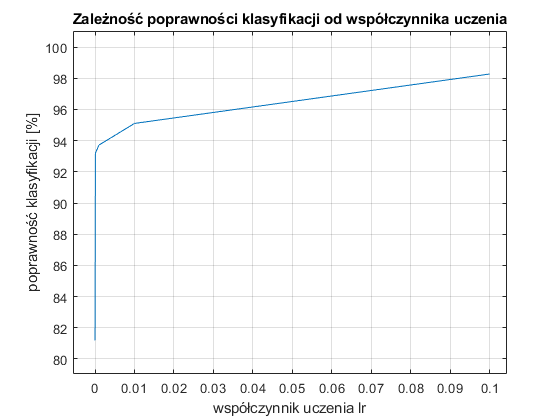
\includegraphics[width=9cm]{srednia pk}
	\caption{Wykres zależności poprawności klasyfikacji od współczynnika uczenia dla średnich ze wszystkich kombinacji ilości neuronów}
\label{Fig:lr1 sse dane}
\end{figure}
\begin{figure}[ht]
	\centering
	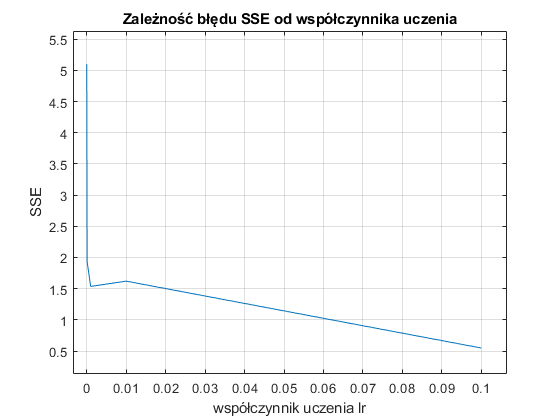
\includegraphics[width=9cm]{srednia sse}
	\caption{Wykres zależności sumy kwadratów błędów od współczynnika uczenia dla średnich ze wszystkich kombinacji ilości neuronów}
\label{Fig:lr1 sse dane}
\end{figure}

\clearpage

\subsubsection{Współczynnik uczenia dla optymalnej ilości neuronów}

Zbadany również został wpływ współczynnika uczenia na poprawność klasyfikacji oraz sumę kwadratów błędów przy optymalnie dobranych ilościach neuronów na warstwie pierwszej i drugiej: S1 = 36, S2 = 21. Działanie skryptu nie wymaga tłumaczenia, ponieważ  bazuje na poprzednich umieszczonych w raporcie kodach - różni się jedynie wartościami w niektórych miejscach, ale zasada działania jest identyczna.

\begin{lstlisting}[frame=single, caption=Skrypt do analizy dotyczącej wpływu wartości współczynnika uczenia przy ustalonej ilości neuronów na uczenie sieci]
%wyczyszczenia środowiska i ustawienie wartości początkowych
close all
clear
disp_freq = 100;
max_epoch = 40000;
max_fail = 10000;
load iris
%ustawienie optymalnej ilości neuronów
S1=36;
S2=21;
%stworzenie potrzebnych tablic
Ptest = zeros([4,30]);
Plearn = zeros([4,120]);
Ttest = zeros([1,30]);
Tlearn = zeros([1,120]);
results = zeros([1,5]);
errors = zeros([1,5]);
err_goal = 0.25/length(Plearn);%błąd docelowy
j = 0;%j to zmienna odpowiadająca za pokazywanie prograsu uczenia

for tries = 1:10 %dla 10 powtórzeń
    i = 0; %zmienne iteracyjne do zapisu wyników w tablicach
    r = 1;
    t = 1;
    for o = 1:3 %podział zbioru na klasy
        [traind] = crossvalind('Holdout', 50, 0.8);    %kroswalidacja danych
        for k = 1:50    %w każdej klasie dane są podzielone na uczące i testujące
           if (traind(k) == 1) %jeżeli indeks jest równy jeden
               %dana jest zapisywana do zbioru testującego
               Ptest(:,t) = Pn(:,k+50*(o-1));
               Ttest(1,t) = T(1,k+50*(o-1));
               t = t + 1;   %iterowanie indeksu
           else
               %w przeciwnym wypadku jest zapisywana do zbioru uczącego
               Plearn(:,r) = Pn(:,k+50*(o-1));
               Tlearn(1,r) = T(1, k+50*(o-1));
               r = r + 1;   %iterowanie indeksu
           end
        end
    end
    for lr = [1e-5, 1e-4, 1e-3, 1e-2, 1e-1]
        j = j + 1;  %zwiększanie progresu uczenia
        i = i + 1;  %zwiększenie zmiennej iteracyjnej
        net = feedforwardnet([S1, S2],'traingd');   %definicja percepton
        net.trainParam.epochs = max_epoch;  %maksymalna liczba epok
        net.trainParam.goal = err_goal; %cel wydajności
        net.trainParam.lr = lr; %learning rate
        net.trainParam.max_fail = max_fail; %maksymalna ilość błędów walidacji
        net.trainParam.showWindow = false;  %czy pokazać okno uczenia
        net.divideParam.trainRatio=1;   %ilość danych do uczenia
        net.divideParam.valRatio=0; %ilość danych do walidacji
        net.divideParam.testRatio=0;    %ilość danych do testowania
        [net,tr] = train(net,Plearn,Tlearn); %uczenie sieci neuronowej
        u = net(Ptest); %zapisanie do u tablicy otrzymanych wyjść
        errors(i) = errors(i) + sse(net, Ttest, u); %zapisanie do errors SSE
        results(i) = results(i) + (1-sum(abs(Ttest-u)>=0.5)/length(Ttest))*100;   %zapisanie do result PK
        process = j/0.5;    %obliczenie progresu
        fprintf('progress: %.2f%%\n', process); %wyświetlenie progresu
    end
end

%obliczenie średnich wyników
results = results / 10;
errors = errors / 10;
%tablica do osi
LRrange = [1e-5, 1e-4, 1e-3, 1e-2, 1e-1];

%wyrysowanie wykresów
figure(1);
plot(LRrange,results);
title('Zależność poprawności klasyfikacji od współczynnika uczenia');
xlabel('współczynnik uczenia lr');
ylabel('poprawność klasyfikacji [%]');
grid;

figure(2);
plot(LRrange,errors);
title('Zależność błędu SSE od współczynnika uczenia');
xlabel('współczynnik uczenia lr');
ylabel('SSE');
grid;
\end{lstlisting}

\clearpage
Otrzymane wykresy mają bardzo podobny charakter do poprzednich, potwierdzają więc, że dla tej sieci zwiększając poprawność klasyfikacji uzyskuje się lepsze wynik. Jedyną różnicą jest tutaj to, że dla lr = 1e-2 SSE nie jest mniejsze, niż dla lr = 1e-3, ale jest to nieistotne dla badania, i nie wpływu na ostateczny kształt wniosków wypływających z tych dwóch eksperymentów.

\begin{figure}[ht]
	\centering
	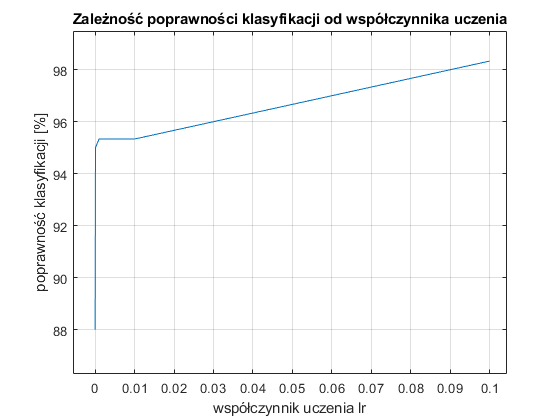
\includegraphics[width=9cm]{3621 pk}
	\caption{Wykres zależności poprawności klasyfikacji od współczynnika uczenia dla dobranych wcześniej 36 neuronów na pierwszej i 21 na drugiej warstwie}
\label{Fig:lr1 sse dane}
\end{figure}

\begin{figure}[ht]
	\centering
	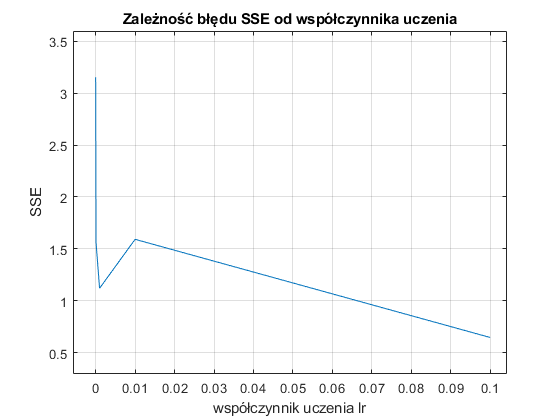
\includegraphics[width=9cm]{3621 sse}
	\caption{Wykres zależności sumy kwadratów błędów od współczynnika uczenia dla dobranych wcześniej 36 neuronów na pierwszej i 21 na drugiej warstwie}
\label{Fig:lr1 sse dane}
\end{figure}

\clearpage

\section{Wnioski}
Dzięki znormalizowaniu danych i przeprowadzeniu serii eksperymentów udało się znaleźć pary liczb określających ilość neuronów na dwóch warstwach sieci, dla których wartości poprawności klasyfikacji osiągały 100\%, a sumy kwadratów błędów 0, co jest wynikiem bardzo zadowalającym. Widać wówczas już było, że najlepsze wyniki sieć osiągała dla współczynnika uczenia rownego lr = 0.1. Po dokładniejszych badaniach udało się określić pożądane wartości pozostałych parametrów: 36 neuronów w pierwszej warstwie, 21 neuronów w drugiej warstwie - dawały one maksymalne Pk i minimalne SSE . Przykład działania sieci z takimi parametrami został zaprezentowany poniżej. Czerwony wykres obrazuje pożądane wyjście sieci, zielony natomiast odpowiadające im otrzymane wyjścia z sieci neuronowej.

\begin{figure}[ht]
	\centering
	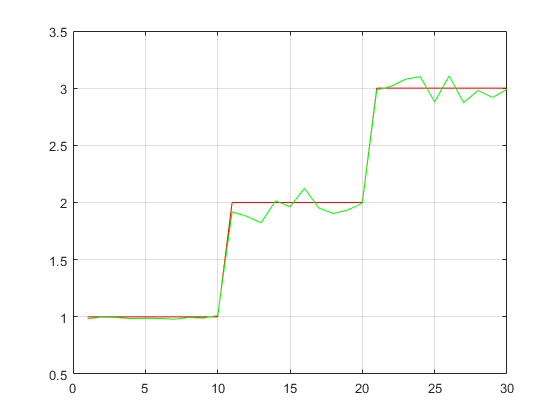
\includegraphics[width=14cm]{zielony}
	\caption{Wykres prównujący wyjście pożądane (docelowe, kolor czerwony) z aktualnym wyjściem sieci (kolor zielony)}
\label{Fig:lr1 sse dane}
\end{figure}

\clearpage
Dla pozostałych parametrów lr można zauważyć, że otrzymane wyniki dla różnych ilości neuronów są bardziej stochastyczne, zakres otrzymywanych wartości zwiększa się, a same wartości maleją wraz ze zmniejszaniem współczynnika uczenia. Warto zauważyć, że ilość neuronów na drugiej warstwie zdaje się być bardziej istotna, niż ich ilość na warstwie pierwszej. Otrzymane dla tych parametrów wartości mogą być podstawą dla dalszych rozważań, w których można zbadać wpływ innych parametrów sieci (np. maksymalna ilość epok) na poprawność klasyfikacji, oraz to, czy zmieniając je udałoby się tę poprawność zwiększyć.\\
Podczas badania współczynnika uczenia nie udało się osiągnąć poprawności klasyfikacji równej 100\% i sumy kwadratów błędów 0 - zarówno wtedy, gdy wartości te były średnimi dla wszystkich par S1 i S2 z zakresu, jak i wtedy, kiedy badano lr dla pożądanych ilości neuronów. W obu przypadkach dla kolejnych wartości lr poprawność klasyfikacji rosła, a suma kwadratów błędów malała, jednak nie osiągały maksimum i minimum. Ten fakt może być podstawą do kolejnych eksperymentów, w których można by badać, czy nadal zwiększając współczynnik uczenia udałoby się osiągnąć lepsze rezultaty.


\clearpage

\addcontentsline{toc}{section}{Literatura}

\begin{thebibliography}{4}
\bibitem{book1} Kosiński, Robert: Sztuczne sieci neuronowe. Dynamika nieliniowa i chaos. 2014. – ISBN 978–83–7926–221–2
\bibitem{str1} MathWorks: Generate indices for training and test sets. \url{https://in.mathworks.com/help/bioinfo/ref/crossvalind.html?s_tid=srchtitle}
\bibitem{str2} MathWorks: Gradient descent backpropagation. \url{https://in.mathworks.com/help/deeplearning/ref/traingd.html?s_tid=mwa_osa_a}
\bibitem{book4} Roman Zajdel, dr hab. inż. prof. PRz .: Sztuczna inteligencja, Laboratorium, Ćwiczenie 6. Model neuronu
\bibitem{book5} Roman Zajdel, dr hab. inż. prof. PRz .: Sztuczna inteligencja, Laboratorium, Ćwiczenie 8. Sieć jednokierunkowa jednowarstwowa
\bibitem{book6} Roman Zajdel, dr hab. inż. prof. PRz .: Sztuczna inteligencja, Laboratorium, Ćwiczenie 9. Sieć jednokierunkowa wielowarstwowa
\bibitem{book7} Zocca, Valentino ; Spacagna, Gianmario ; Slater, Daniel ; Roelantsi, Peter: Deep Learning. Uczenie głębokie z językiem Python. Sztuczna inteligencja i sieci neuronowe. 2018. –  ISBN 978–83–283–4174–6
\end{thebibliography}

\clearpage

\end{document} 
